\section{Introduction}

Traditionally, circuit switching and packet switching have been
considered as alternative design choices, each with their own advantages
and disadvantages. Packet switches are efficient at multiplexing traffic
across a large number of ports, while circuit switches can often service
higher line rates in a more cost-effective manner, especially when
combined with optical links. However, as optical circuit switching
technology advances, the reconfiguration time (i.e., the amount of time
it takes to alter the input-to-output mapping) is swiftly decreasing,
thus increasingly blurring the division between the packet and circuit
regimes.

One key domain in which these design tradeoffs are being revisited today
is datacenter switching. The datacenter environment, aggregating
tremendous amounts of compute and storage capacity, has driven demand
for ever increasing port counts and line speeds. However, supporting
these demands with existing packet switching technology is becoming
increasingly expensive—in cost, heat and power. Moreover, studies have
shown that the traffic demand inside a datacenter (both within and
across racks) is frequently highly nonuniform, with a large fraction of
the traffic at each switch port destined for a small number of output
ports~\cite{Kandula:2009-2}.

Based on these observations, researchers had proposed hybrid datacenter
network architectures that offer higher throughputs at lower cost by
combining switching technologies. In particular, recent proposals
suggest employing highspeed optical~\cite{Chen:2012, Farrington:2010,
Wang:2010} or wireless~\cite{Halperin:2011, Kandula:2009, Zhou:2012}
networks configured to service the heavy flows, while passing the
remainder of the traffic through a traditional, relatively
underprovisioned packet-switched network. 

As technology trends usher in dramatically faster reconfiguration times,
the distinction between packet and circuit is blurred, and ever smaller
flows can take advantage of a hybrid fabric. This trend will soon allow
servicing the bulk of the traffic through a rapidly reconfigurable
optical switch~\cite{Porter:2013}, leaving a relatively minor portion to
be serviced by the packet network~\cite{Liu:2014}. While the potential
cost savings that hybrid technologies could realize is large, the design
space for scheduling resources in the hybrid regime is not yet well
understood. 

Many of the classical approaches to scheduling for switches with
non-trivial reconfiguration delays divide the offered demand into two
parts: an initial, heavy-weight component that is served by O(N) highly
utilized configurations with significant durations, and a second,
residual component that is serviced by a similar number of short,
under-utilized schedules. Recent Solstice scheduling
algorithm~\cite{Liu:2014} exploits the skewed nature of datacenter
traffic patterns to create a small number of configurations with long
durations that minimize the penalty for reconfiguration and leaves only
a small amount of residual demand to be serviced by a low-speed (and
lowcost) unconstrained packet switch.

To ensure high overall circuit utilization, each circuit configuration
must be maintained for a relatively long period with respect to the
reconfiguration delay. This leads to two issues for the scheduling
algorithm: Since the demand is skewed, the demands served by a single
configuration could have a large variation. Thus a portion of the links
in optical switch could be under-utilized. Since the configuration time
is still non-trivial, it is still hard to schedule small traffic demands
efficiently on optical switch. Scheduling algorithms are forced to serve
these small demands by packet switch, which is slower and less
cost-effective.

To increase the utilization rate of the optical switches and to reduce the
number of configurations, we propose an indirection scheduling technique: instead
of scheduling each demand with unique direct path, we could leverage existing
paths to serve some demands indirectly. Using this technique, scheduling algorithm
could reduce the skewness of the demands and reduce the number of configurations.

The evaluation of the indirection technique has two objectives. The
first is to find out the optimal possible benefit of indirection. We
achieved this goal by formulating the scheduling problem into an integer
linear programming (ILP) problem. Using $Gurobi$ ILP
solver~\cite{Gurobi} to compare the optimal solution with and without
indirection, we show that using indirection could reduce the number of
configurations and the total transmission time.

The second objective is to find out the practical benefit of indirection.
We achieved this goal by simulations of hybrid switch scheduling. We implemented
two simple indirection heuristics and applied them to the Solstice algorithm.
Comparing the simulations of Solstice algorithm with and without
indirection heuristics, results show that even simple indirection
heuristics could provide improvements above direct path algorithm.
Although our indirection heuristics didn't approach similar amount
of improvement as in the ILP formulation results, we argue that better
improvement is possible with clever indirection heuristics embedded with
the scheduling algorithm.

The rest of this report is organized as follows. Section~\ref{sec:ilp}
described the ILP formulation and the solver results.
Section~\ref{sec:simres} describes the preliminary indirection
heuristics and the simulation results. Finally, we summarize this
project in Section~\ref{sec:conclusion}.

\section{ILP Formulation of the Scheduling Problem}
\label{sec:ilp}

\subsection{Problem Formulation}
Integer linear programming is a mathematical optimization method. An
integer linear program is expressed with a minimization/maximization
objective function, constraints of the variables, and bounds of the
variables. For our scheduling problem, the objective function is clearly
the minimization of the total transmission time, but the constraints are
complicated. In the remaining of this section, we will describe the
constraints implemented in the program.

\paragraph{Input Demand Matrix}
To define the input of each integer linear program, we defined the demands
needs to be served as a N by N matrix, where N is the number of ports in the
network. Entry (a, b) in the input demand matrix denotes the amount of demand
to be transfered from port a to port b. Each (a, a) entry has zero demand.
Then we ask the program to solve the scheduling problem so that each demand in
the input demand matrix must be served by either optical or packet switch.

\paragraph{Optical Switch Constraints}
To define the optical switch, we need to implement the concept of configurations.
Each configuration is a matrix that denotes the demands served by this
configuration. Since the input-output mapping is fixed in a single configuration,
each row and each column can only have no more than one non-zero entry.
For each new configuration scheduled, an additional reconfiguration time
is added to the total transmission time. 

\paragraph{Packet Switch Constraints}
Packet switch constraints are different. Packet switch doesn't have the concept
of configurations. It could schedule arbitrary amount of demands on each link
without any reconfiguration time. However, packet switch has less capacity than
optical switch. Thus it could only schedule a smaller fraction of demands within
the same time duration. In our constraints, we configure the packet switch to
have $1/10$ capacity of the optical switch. 

\paragraph{Indirection Technique Constraints}  
To define the indirection technique, we defined each possible indirection decision
in the program. If a decision is made that certain amount of demand from port a
to port b will be indirectly served by paths a -> c and c -> b, the input demand matrix
will reduce the demand in entry (a, b) and increase the demands in entries (a, c)
and (c, b). 

\subsection{ILP Solving Results}

\begin{table}
\centering
{
\begin{tabular}{l|r|r|r|r}
\toprule
\bf Optimal Total Time & \bf Random $\delta$ = 5 & \bf Random $\delta$ = 10 & \bf Random $\delta$ = 20 & \bf Skewed $\delta$ = 10 \\
\midrule
Orig & 100\% & 100\% & 100\% & 100\% \\
Indi & 93.93\% & 90.65\% & 83.8\% & 97.9\% \\
\bottomrule
\end{tabular}
}
\caption{Normalized average optimal solution achieved by direct path scheduling (Orig) and indirection technique (Indi), $\delta$ is the reconfiguration time.}
\label{tab:ilp}
\end{table}

\begin{figure}
	\centering
	\begin{minipage}{3in}%
		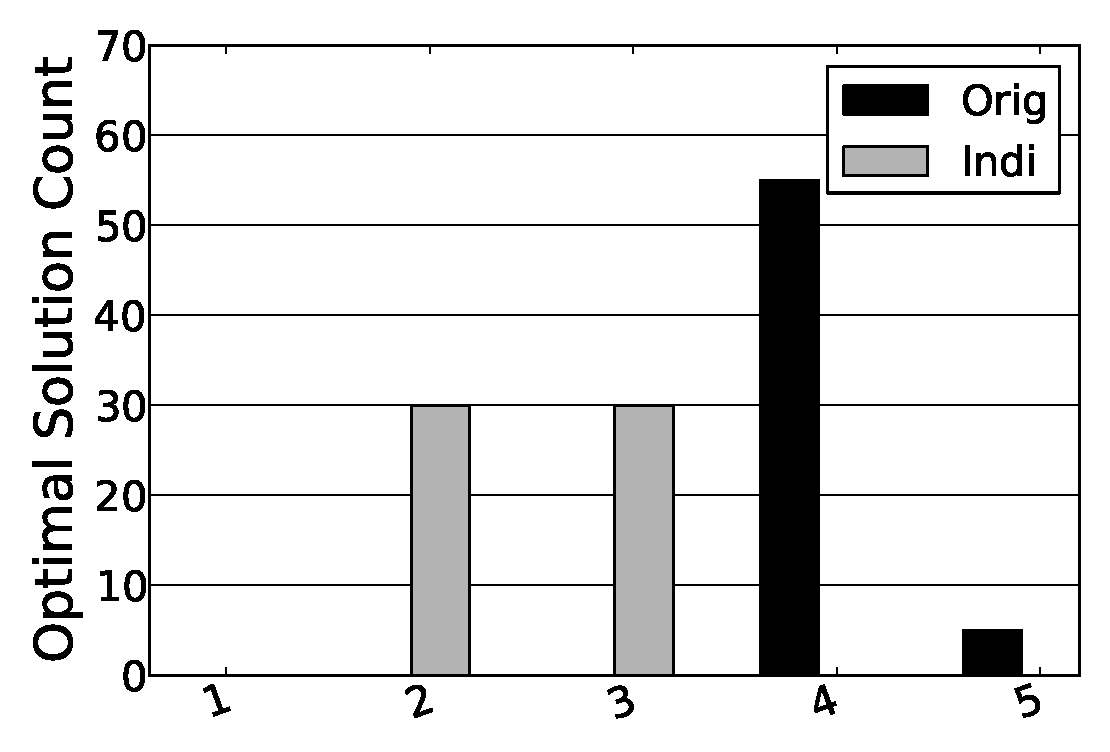
\includegraphics[width=3in]{figures/avg-5-rand}
		\caption{Optimal solution count for different number of configurations with random demand}
		\label{fig:5rand}
	\end{minipage}%
	\qquad
	\begin{minipage}{3in}%
		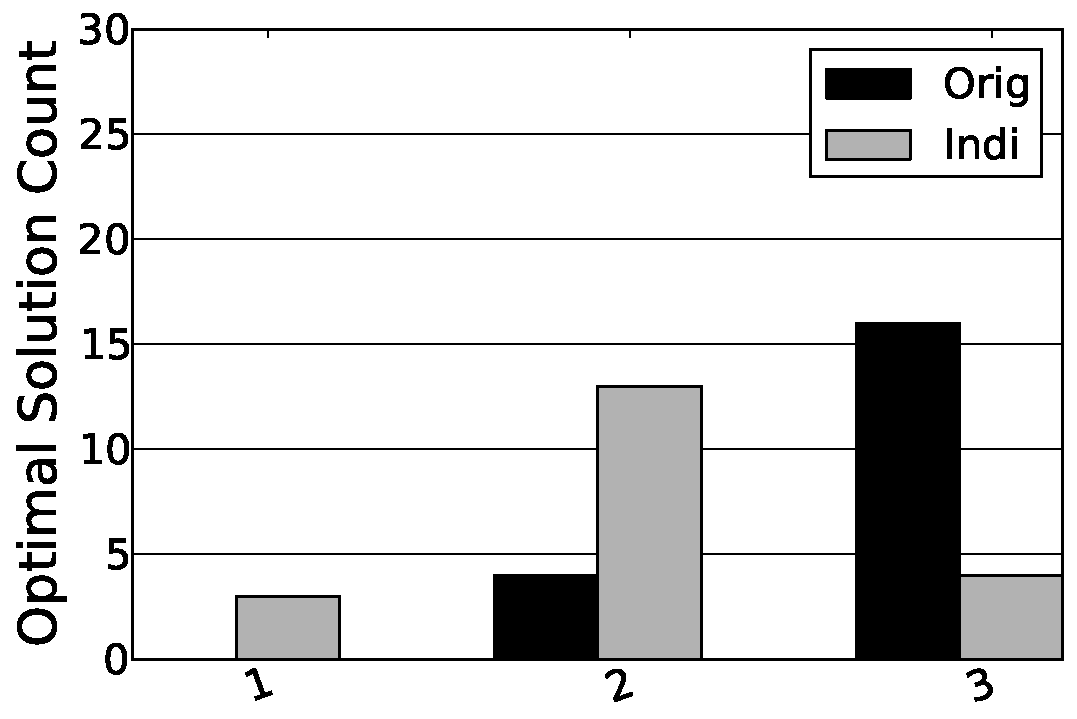
\includegraphics[width=3in]{figures/avg-5-skew}
		\caption{Optimal solution count for different number of configurations with skewed demand}
		\label{fig:5skew}
	\end{minipage}%
\end{figure}

We used the Gurobi ILP solver to solve the optimal solutions of our
integer linear programs. Since integer linear solving is NP-hard, we
choose to solve 5 by 5 input demand matrix. This is a small input
compared to the matrix used in the simulator. But it is big enough to
show the potential benefit of the indirection technique.

We used two different kinds of workload. The first is random workload
where each entry has a demand randomly chosen from 0 to 40. To show the
effect of the reconfiguration time, we tested different reconfiguration
times between 5 to 20 for the random workload. The second workload is
skewed workload where each port sends one big demand (around 250) and
two small demand (around 40). For this workload, we only tested with
reconfiguration time as 10. 

We generated 20 integer linear programs with different input demand
matrices for each workload and each reconfiguration time used. Then we
let the Gurobi solver to solve these programs and report the optimal
solutions. Table~\ref{tab:ilp} shows the normalized average optimal
solutions for each workload and different reconfiguration time.
Indirection technique provides improvement for all workloads. In
particular, indirection provides more improvements when the ratio of
demand to reconfiguration time is smaller. This is because indirection
technique helps on reducing the number of configurations.
Figure~\ref{fig:5rand} and Figure~\ref{fig:5skew} depict the number of
configurations needed for each optimal solution for both with and
without indirection. Results show that indirection technique reduced the
number of configurations for most of test cases.